\section{Derivadas para Funções de Duas Variáveis}

	\subsection{Derivadas Parciais \cite{morettin}}

		Consideremos um ponto $(x_{0}, y_{0})$; se mantivermos $y$ constante no valor $y_{0}$ e variarmos $x$ do valor $x_{0}$ para  o valor $x_{0} + \Delta x$, a função $f(x_{0}, y_{0})$ dependerá apenas da variável $x$.

		\medskip

		Seja

		\bigskip

		$\Delta f = f(x_{0} + \Delta x, y_{0}) - f(x_{0}, y_{0})$.

		\bigskip

		À razão
		
		\bigskip
		
		$\cfrac{\Delta f}{\Delta x} = \cfrac{f(x_{0} + \Delta x, y_{0}) - f(x_{0}, y_{0})}{\Delta x}$.

		\bigskip

		chamamos de taxa média de variação de $f$ em relação a $x$.

		\medskip

		Observemos que:
		
		\begin{enumerate}[label=(\alph*)]

			\item $\cfrac{\Delta f}{\Delta x}$ depende do ponto de partida $(x_{0}, y_{0})$;
			\item $\cfrac{\Delta f}{\Delta x}$ depende da variação $\Delta x$.

		\end{enumerate}

		Ao limite (se existir e for um número real) de $\cfrac{\Delta f}{\Delta x}$ , quando $\Delta x$ tende a $0$, denominamos derivada parcial de $f$ no ponto $(x_{0}, y_{0})$, em relação a $x$. Indicamos a tal derivada parcial por um dos símbolos:

		\bigskip

		$\cfrac{\partial f}{\partial x} (x_{0}, y_{0})$ \ \ \ ou \ \ \ $f_{x}(x_{0}, y_{0})$ .
		
		\bigskip

		Assim,

		\bigskip

		{\LARGE $\cfrac{\partial f}{\partial x} (x_{0}, y_{0}) = f_{x}(x_{0}, y_{0}) = \lim \limits_{\Delta x \to 0} \cfrac{\Delta f}{\Delta x}$} .

		\bigskip

		O símbolo $\cfrac{\partial f}{\partial x}$ (lê-se del $f$, del $x$) foi introduzido por Lagrange (Joseph Louis Lagrange, 1736-1813, matemático nascido na Itália, mas que viveu a maior parte da vida na França).

		Analogamente, se mantivermos $x$ constante no valor $x_{0}$ e variarmos $y$ do valor $y_{0}$ para o valor $y_{0} + \Delta y$, $f$ dependerá apenas da variável $y$.

		\medskip

		Seja

		\bigskip

		$\Delta f = f(x_{0}, y_{0} + \Delta y) - f(x_{0}, y_{0})$.

		\bigskip

		À razão
		
		\bigskip
		
		$\cfrac{\Delta f}{\Delta y} = \cfrac{f(x_{0}, y_{0} + \Delta y) - f(x_{0}, y_{0})}{\Delta y}$.

		\bigskip

		chamamos de taxa média de variação de $f$ em relação a $y$.

		Ao limite (se existir e for um número real) de $\cfrac{\Delta f}{\Delta y}$ quando $\Delta y$ tente a $0$, denominamos derivada parcial de $f$ no ponto $(x_{0}, y_{0})$, em relação a $y$. Indicamos tal derivada parcial por um dos símbolos:

		\bigskip

		$\cfrac{\partial f}{\partial y} (x_{0}, y_{0})$ \ \ \ ou \ \ \ $f_{y}(x_{0}, y_{0})$ .

		\bigskip

		O símbolo $\cfrac{\partial f}{\partial y}$ (lê-se del $f$, del $y$).

		\bigskip

		Assim,

		\bigskip

		{\LARGE $\cfrac{\partial f}{\partial y} (x_{0}, y_{0}) = f_{y}(x_{0}, y_{0}) = \lim \limits_{\Delta y \to 0} \cfrac{\Delta f}{\Delta y}$} .

		\bigskip

		\textbf{Exemplo 10.1}. Seja $f(x, y) = 2x +3y$. Calculemos $\cfrac{\partial f}{\partial x} (4, 5)$ e $\cfrac{\partial f}{\partial y} (4, 5)$.

		\medskip

		Temos:

		\medskip

		$\cfrac{\partial f}{\partial x} (4, 5) = \lim \limits_{\Delta x \to 0} \cfrac{f(4 + \Delta x, 5) - f(4, 5)}{\Delta x}$

		$\cfrac{\partial f}{\partial x} (4, 5) = \lim \limits_{\Delta x \to 0} \cfrac{2(4 + \Delta x) + 3 \times 5 - 2 \times 4 + 3 \times 5}{\Delta x}$

		$\cfrac{\partial f}{\partial x} (4, 5) = \lim \limits_{\Delta x \to 0} \cfrac{2 \times \Delta x}{\Delta x} = 2$
		
		\medskip

		Analogamente,

		\medskip

		$\cfrac{\partial f}{\partial y} (4, 5) = \lim \limits_{\Delta y \to 0} \cfrac{f(4, 5 + \Delta y) - f(4, 5)}{\Delta y}$

		$\cfrac{\partial f}{\partial y} (4, 5) = \lim \limits_{\Delta y \to 0} \cfrac{2 \times 4 + 3 \times (5 + \Delta y) - 2 \times 4 + 3 \times 5}{\Delta y}$

		$\cfrac{\partial f}{\partial y} (4, 5) = \lim \limits_{\Delta y \to 0} \cfrac{3 \times \Delta y}{\Delta y} = 3$	
		
	\subsection{Função Derivada Parcial \cite{morettin}}

		Se calcularmos $f_{x}$ e $f_{y}$ num ponto genérico $(x, y)$, obteremos duas funções de $x$ e $y$; a função $f_{x}(x, y)$ é chamada função derivada parcial de $f$ em relação a $x$ (ou, simplesmente, \textbf{derivada parcial de $f$ em relação a $x$}). A função $f_{y}(x, y)$ é chamada função derivada parcial de $f$ em relação a $y$ (ou, simplesmente, \textbf{derivada parcial de $f$ em relação a $y$}). As derivadas parciais também podem ser indicadas por

		\bigskip

		{\LARGE $f_{x} \ \text{ou} \ \cfrac{\partial f}{\partial x}$ \ \ \ ou \ \ \ $f_{y} \ \text{ou} \ \cfrac{\partial f}{\partial y}$} .
		
		\bigskip

		Para o cálculo de $f_{x}$ e $f_{y}$, podemos aplicar as regras de derivação estudadas em funções de uma variável, desde que:

		\begin{enumerate}[label=(\alph*)]

			\item no cálculo de $f_{x}$ consideremos $y$ como constante;
			\item no cálculo de $f_{y}$ consideremos $x$ como constante.

		\end{enumerate}
		
	\subsection{Diferencial de uma Função - Derivada/Diferencial Total \cite{morettin}}

		Consideremos a função dada por $f(x, y) = 2x^{2} + 3x^{2}$, e calculemos a variação $\Delta f$ sofrida pela função quando $x$ e $y$ sofrem variações $\Delta x$ e $\Delta y$ a partir do ponto $(x_{0}, y_{0})$.

		\medskip

		Temos:

		\medskip

		$\Delta f = f(x_{0} + \Delta x, y_{0} + \Delta y) - f(x_{0}, y_{0})$

		$\Delta f = 2(x_{0} + \Delta x)^{2} + 3(y_{0} + \Delta y)^{2} - (2x^{2}_{0} + 3y^{2}_{0})$

		$\Delta f = 2(x^{2}_{0} + 2x_{0}\Delta x + \Delta x^{2}) + 3(y^{2}_{0} + 2y_{0}\Delta y + \Delta y^{2}) - 2x^{2}_{0} - 3y^{2}_{0}$

		$\Delta f = 4x_{0}\Delta x + 6y_{0}\Delta y + 2\Delta x^{2} + 3\Delta y^{2}$ .

		\medskip

		Por exemplo, se $x_{0} = 5$, $y_{0} = 6$ e $\Delta x = \Delta y = 0,01$, teremos:

		\medskip

		$\Delta f = 4 \times (5) \times 0,01 + 6 \times (6) \times 0,01 + 2(0,01)^{2} + 3(0,01)^{2}$

		$\Delta f = 0,2 + 0,36 + 0,0002 + 0,0003$ .

		\medskip

		Como as parcelas $0,0002$ e $0,0003$ são desprezíveis comparadas com $0,02$ e $0,36$, podemos dizer que

		\medskip

		$\Delta f \cong 0,2 + 0,36 = 0,56$ .

		\medskip

		Voltando à expressão de $\Delta f$, notamos que:

		\begin{itemize}

			\item $4x_{0} = \cfrac{\partial f}{\partial x} (x_{0}, y_{0})$ e $6y_{0} = \cfrac{\partial f}{\partial y} (x_{0}, y_{0})$

			\item Os termos $2\Delta x^{2} + 3\Delta y{2}$ são desprezíveis quando comparados com $4x_{0}\Delta x + 6y_{0}\Delta y$, \textbf{desde que $\Delta x$ e $\Delta y$ sejam próximos de zero};

			\item $\Delta f \cong \cfrac{\partial f}{\partial x} (x_{0}, y_{0}) \times \Delta x + \cfrac{\partial f}{\partial y} (x_{0}, y_{0}) \times \Delta y$ .

		\end{itemize}

		O resultado que acabamos de ver não é um caso isolado, mas vale para a grande maioria das funções, isto é, a variação sofrida por $f(x, y)$ quando variamos simultaneamente $x$ e $y$ de \textbf{valores pequenos $\Delta x$ e $\Delta y$} é aproximadamente igual a $\cfrac{\partial f}{\partial x} (x_{0}, y_{0}) \times \Delta x + \cfrac{\partial f}{\partial y} (x_{0}, y_{0}) \times \Delta y$.

		Esse exemplo preliminar nos leva à seguinte definição.

		Seja $f$ uma função com duas variáveis e seja $(x_{0}, y_{0})$ um ponto de seu domínio. Seja $\Delta f$ a variação sofrida por $f(x, y)$ ao passarmos do ponto $(x_{0}, y_{0})$ para o ponto $(x_{0} + \Delta x, y_{0} + \Delta y)$. Isto é,

		\medskip

		$\Delta f = (x_{0} + \Delta x, y_{0} + \Delta y) - f(x_{0}, y_{0})$ .

		\medskip

		Dizemos que $f$ é \textbf{diferenciável no ponto $(x_{0}, y_{0})$} se $\Delta f$ puder ser escrita sob a forma

		\medskip

		$\Delta f = \cfrac{\partial f}{\partial x} (x_{0}, y_{0}) \times \Delta x + \cfrac{\partial f}{\partial y} (x_{0}, y_{0}) \times \Delta y + \Delta x \times h_{1}(\Delta x, \Delta y) + \Delta y \times h_{2}(\Delta x, \Delta y)$,

		\medskip

		em que as funções $h_{1}$ e $h_{2}$ têm limites iguais a zero quando $(\Delta x, \Delta y)$ tende a $(0, 0)$.

		\medskip

		A parcela $\cfrac{\partial f}{\partial x} (x_{0}, y_{0}) \times \Delta x + \cfrac{\partial f}{\partial y} (x_{0}, y_{0}) \times \Delta y$ é chamada diferencial de $f$ e é indicada por $df$, no caso de $f$ ser diferenciável.

		\bigskip

		{\LARGE $df = \cfrac{\partial f}{\partial x} (x_{0}, y_{0}) \times \Delta x + \cfrac{\partial f}{\partial y} (x_{0}, y_{0}) \times \Delta y$}

		\bigskip

		Voltando ao exemplo inicial, vimos que

		\medskip

		$\Delta f = 4x_{0}\Delta x + 6y_{0}\Delta y + 2\Delta x^{2} + 3\Delta y^{2}$ .

		\medskip

		Assim, como

		\medskip

		$4x_{0} = \cfrac{\partial f}{\partial x} (x_{0}, y_{0})$,

		$6y_{0} = \cfrac{\partial f}{\partial y} (x_{0}, y_{0})$.

		\medskip

		$h_{1}(\Delta x, \Delta y) = 2\Delta x$ e $h_{2}(\Delta x, \Delta y) = 3\Delta y$, ambas com limites nulos quando $(\Delta x, \Delta y)$ tendem a $(0, 0)$, concluímos que $f$ é diferenciável num ponto genérico $(x_{0}, y_{0})$.

		\subsubsection{Teorema \cite{morettin}}

			Seria bastante trabalho termos que verificar pela definição se uma função é ou não diferenciável, para podermos calcular a diferencial como resultado aproximado de $\Delta f$. Felizmente, existe um teorema que nos fornece condições facilmente verificáveis para vermos se função é diferenciável. Seu enunciado é o seguinte:

			Seja $f$ uma função com duas variáveis. Se as derivadas $\cfrac{\partial f}{\partial x}$ e $\cfrac{\partial f}{\partial y}$ são contínuas num conjunto aberto $A$, então $f$ é diferenciável em todos os pontos de $A$.

			\bigskip

			\textbf{Exemplo}. A função $f(x, y) = 2x^{2} + 4y^{3}$ é diferenciável em todos os pontos de $\mathbb{R}^{2}$, pois as derivadas parciais $\cfrac{\partial f}{\partial x} = 4x$ e $\cfrac{\partial f}{\partial y} = 12y^{2}$ são contínuas em $\mathbb{R}^{2}$. A diferencial de $f$ num ponto genérico $(x, y)$ vale

			\bigskip

			$df = 4x \times \Delta x + 12y^{2} \times \Delta y$ .

			\medskip

			\textbf{Exemplo}. A função $f(x, y) = \cfrac{2x}{x - y}$ com domínio $D = \{(x, y) \in \mathbb{R}^{2} \mid x \neq y\}$ é diferenciável em $D$, pois as derivadas parciais $\cfrac{\partial f}{\partial x} = \cfrac{-2x}{(x - y)^{2}}$ \ e \ $\cfrac{\partial f}{\partial y} = \cfrac{2x}{(x - y)^{2}}$ são contínuas em $D$. A diferencial de $f$ num ponto genérico $(x, y)$ vale

			\medskip

			$df = \cfrac{-2x}{(x - y)^{2}} \times \Delta x +  \cfrac{2x}{(x - y)^{2}} \times \Delta y$ .

	\subsection{Função Composta - Regra da Cadeia \cite{morettin}}

		Consideremos uma função de produção $P(x, y) = 6x^{0,5} \times y^{0,5}$ em que $x$ e $y$ são as quantidades de dois insumos, capital e trabalho, e $P$, a quantidade produzida de um produto.

		Suponhamos que o capital $x$ cresça com o tempo $t$, de acordo com a relação $x = 0,16t$, e o trabalho cresça de acordo com a relação $y = 0,09t$.

		Se quisermos expressar a produção em função do tempo, temos que substituir $x = 0,16t$ e $y = 0,09t$ na relação $P(x, y) = 6x^{0,5} \times y^{0,5}$. Procedendo dessa forma teremos:

		\medskip

		$P(t) = 6(0,16t)^{0,5} \times (0,09t)^{0,5} = 0,72t$ .

		\medskip

		À função de $t$, dada por $P(t) = 0,72t$, chamamos de \textit{função composta} de $P$ com $x$ e $y$.

		A derivada da função composta dada por $P(t) = 0,72t$ em relação a $t$ é imediata (função de uma variável):

		\medskip

		$P'(t) = \cfrac{dP}{dt} = 0,72$.

		\medskip

		Isso é, a taxa de crescimento do produto em relação ao tempo é $0,72$.

		De modo geral, a derivada da função composta pode ser obtida facilmente por mera substituição e derivação da função de uma variável, como vimos no exemplo. Entretanto, existe um fórmula alternativa de cálculo da derivada da função composta, conhecida como regra da cadeira, que veremos a seguir.

		\subsubsection{Teorema - Regra da Cadeia \cite{morettin}}

			Seja $f$ uma função de duas variáveis $x$ e $y$, diferenciável num ponto $(x_{0}, y_{0})$ do domínio, e sejam as funções dadas por $x(t)$ e $y(t)$ diferenciáveis em $t_{0}$, de modo que $x(t_{0}) = x_{0}$ e $y(t_{0}) = y_{0}$. Então a função $F$ composta de $f$ com $x$ e $y$ é tal que:

			\bigskip

			{\LARGE $\cfrac{dF}{dt}(t_{0}) = \cfrac{\partial f}{\partial x}(x_{0}, y_{0}) \times \cfrac{dx}{dt}(t_{0}) + \cfrac{\partial f}{\partial y}(x_{0}, y_{0}) \times \cfrac{dy}{dt}(t_{0})$},

			\bigskip

			ou abreviadamente

			\medskip

			$\cfrac{dF}{dt} = \cfrac{\partial f}{\partial x} \times \cfrac{dx}{dt} + \cfrac{\partial f}{\partial y} \times \cfrac{dy}{dt}$
			
	\subsection{Funções Definidas Implicitamente \cite{morettin}}

	\subsection{Funções Homogêneas - Teorema de Euler \cite{morettin}}

	\subsection{Derivadas Parciais de Segunda Ordem \cite{morettin}}

		Seja uma função de duas variáveis $x$ e $y$, $fx$  e $fy$ suas derivadas parciais. Se calcularmos as derivadas parciais de $fx$ e $fy$, obteremos quatro funções chamadas derivadas parciais de segunda ordem. São elas:

		\begin{enumerate}[label=(\alph*)]

			\item derivada de $fx$ em relação a $x$, indicada por $fxx$ \ ou \ $\cfrac{\partial^{2}f}{\partial x^{2}}$ ;

			\item derivada de $fx$ em relação a $y$, indicada por $fxy$ \ ou \ $\cfrac{\partial^{2}f}{\partial y\partial x}$ ;

			\item derivada de $fy$ em relação a $x$, indicada por $fyx$ \ ou \ $\cfrac{\partial^{2}f}{\partial x\partial y}$ ;

			\item derivada de $fy$ em relação a $y$, indicada por $fyy$ \ ou \ $\cfrac{\partial^{2}f}{\partial y^{2}}$ ;

		\end{enumerate}
		
		É importante observar que $fxy$ e $fyx$ deverão \textbf{sempre} ter iguais valores, caso contrário pode ter ocorrido algum erro nos cálculos \cite{lucchesi}.

	\subsection{Integrais Duplas \cite{morettin}}

		Consideremos uma função de duas variáveis $f(x, y)$ e suponhamos que a derivada parcial em relação a $x$, seja $fx(x, y) = 6xy$.

		Mantendo $y$ como constante e integrando essa derivada parcial em relação a $x$, obtemos a função $f(x, y)$:

		\medskip

		$\int fx(x, y)dx = \int 6xy dx = 3x^{2}y + c(y)$ .

		\medskip

		Assim

		\medskip

		$f(x, y) = 3x^{2}y + c(y)$ .

		\medskip

		A integral calculada é chamada integral parcial a relação a $x$. A constante de integração $c(y)$ é função de $y$, pois $y$ é mantido constante na integração parcial em relação a $x$.

		Caso quiséssemos calcular a integral definida de $fx(x, y)$, com limites de integração entre $0$ e $2y$, teríamos:

		\medskip

		$\int \limits^{2y}_{0} fx(x, y) dx = \int \limits^{2y}_{0} 6xy dx = \left[3x^{2}y\right]^{2y}_{0} = 3(2y)^{2}y - 0 = 12y^{3}$ .

		\medskip

		Analogamente, se em uma função $f(x, y)$ conhecêssemos a derivada parcial em relação a $y$, $fy(x, y) = 2x + y$, o cálculo de $f(x, y)$ seria feito pela integral parcial em relação a $y$, ou seja:

		\medskip

		$f(x, y) = \int fy(x, y) dy = \int (2x + y) dy = 2xy + \cfrac{y^{2}}{2} + c(x)$ ,

		\medskip

		em que $c(x)$ é uma constante que depende de $x$. Caso estivéssemos calculando a integral parcial definida, em relação a $y$, entre os limites $1$ e $x$, teríamos:

		\medskip

		$\int \limits^{x}_{1} (2x + y) dy = \left[ 2xy + \cfrac{y^{2}}{2}\right]^{x}_{1} = 2x(x) + \cfrac{x^{2}}{2} - \left( 2x \times 1 + \cfrac{1^{2}}{2} \right) = \cfrac{5}{2} x^{2} - 2x - \cfrac{1}{2}$ .
		
		\subsubsection{Integral Dupla \cite{morettin}}

			Consideremos uma função $f(x, y)$ não negativa, definida no domínio $D$ constituído do retângulo dado pelas inequações $a \leq x \leq b$ e $c \leq y \leq d$ (Figura 10.4).

			\begin{figure}[H]
				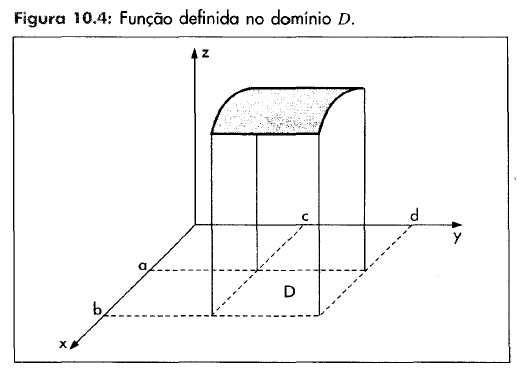
\includegraphics[height=7.5cm]{images/morettin_figura-10-4}
			\end{figure}

			Ao calcularmos a integral parcial (em relação a $y$) $A(x)$, entre $c$ e $d$, estaremos mantendo $x$ constante. Assim, $A(x)$ representará a área da secção do gráfico da função, perpendicular ao eixo $x$, num ponto genérico entre $a$ e $b$. Isto é, $A(x) = \int \limits^{d}_{c} f(x, y)dy$ (Figura 10.5).

			\begin{figure}[H]
				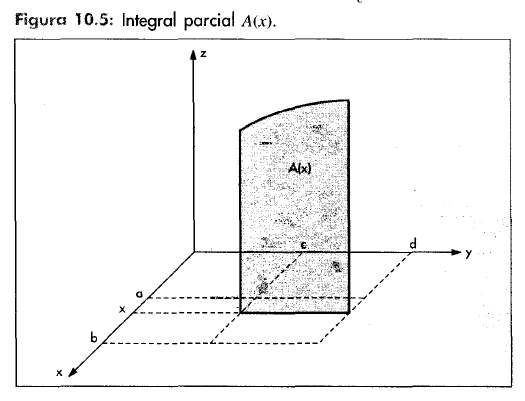
\includegraphics[height=7.5cm]{images/morettin_figura-10-5}
			\end{figure}

			O produto $A(x)dx$ representa o volume do sólido de área $A(x)$ e espessura $dx$. Assim, a integral de $A(x)$ em relação a $x$ representará o volume do sólido sob o gráfico de $f(x, y)$, acima do domínio $D$.

			A esse volume damos o nome de integral dupla de $f(x, y)$ no domínio $D$. Dessa forma, indicando por $V$ o volume do referido sólido, teremos

			\medskip

			$V = \int \limits^{b}_{a} A(x)dx$ .

			\medskip

			Simbolizando a integral dupla por $\int \int_{D} f(x, y)dxdy$, podemos escrever:

			\bigskip

			{\LARGE $\iint_{D} f(x, y)dxdy = \int \limits^{b}_{a} \left[ \int \limits^{d}_{c} f(x, y)dy \right] dx$} . 

			\bigskip

			Poderíamos também ter calculado a área de uma secção perpendicular ao eixo $y$, $B(y)$, da seguinte forma

			\medskip

			$B(y) = \int \limits^{b}_{a} f(x, y)dx$ ,

			\medskip

			e em seguida calculado o volume do sólido sob o gráfico da função e acima do domínio $D$ por

			\medskip

			$V = \int \limits^{d}_{c} B(y)dy = \int \limits^{d}_{c} \left[ \int \limits^{b}_{a} f(x, y)dx \right] dy$ .

			\bigskip

			\textbf{Exemplo}. Consideremos a função $f(x, y) = x + y$, definida no domínio $D$ dado pelas inequações $0 \leq x \leq 5$ e $0 \leq y \leq 3$ e calculemos a integral dupla $\iint _{D} f(x, y)dxdy$, ou seja, o volume $V$ do sólido sob o gráfico da função e acima de $D$.

			\medskip

			a) Primeiro modo

			\medskip

			$A(x) = \int \limits^{3}_{0} (x + y)dy = \left[ xy + \cfrac{y^{2}}{2} \right]^{3}_{0} = 3x + \cfrac{9}{2}$ ,

			$V = \int \limits^{5}_{0} \left( 3x + \cfrac{9}{2} \right) dx = \left[ \cfrac{3x^{2}}{2} + \cfrac{9}{2} x \right]^{5}_{0} = \cfrac{75}{2} + \cfrac{45}{2} = 60$ .

			\bigskip

			b) Segundo modo

			\medskip

			$B(y) = \int \limits^{5}_{0} (x + y)dx = \left[ \cfrac{x^{2}}{2} + xy \right]^{5}_{0} = \cfrac{25}{2} + 5y$ ,

			$V = \int \limits^{3}_{0} \left( \cfrac{25}{2} + 5y \right) dy = \left[ \cfrac{25y}{2} + \cfrac{5y^{2}}{2} \right]^{3}_{0} = \cfrac{75}{2} + \cfrac{45}{2} = 60$.

			\bigskip

			Uma outra situação que ocorre no cálculo da integral dupla é aquela em que o domínio $D$ da função é dado por

			\medskip

			$a \leq x \leq b$

			\smallskip

			e

			\smallskip

			$y_{1}(x) \leq y \leq y_{2}(x)$

			\medskip

			Veja a Figura 10.6.

			\begin{figure}[H]
				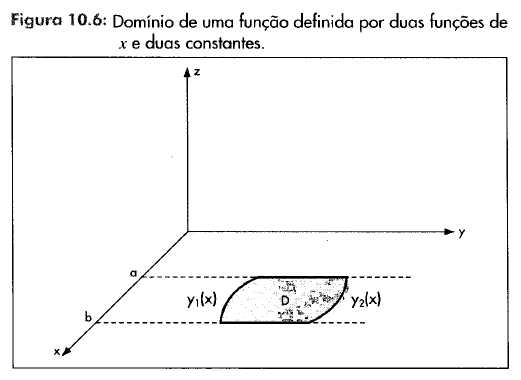
\includegraphics[height=7cm]{images/morettin_figura-10-6}
			\end{figure}

			O $1^{o}$ passo para o cálculo da integral dupla consiste em acha a área $A(x)$ de uma secção do gráfico perpendicular ao eixo $x$, $A(x) = \int \limits^{y_{2}(x)}_{y_{1}(x)} f(x, y)dy$ (Figura 10.7).

			\begin{figure}[H]
				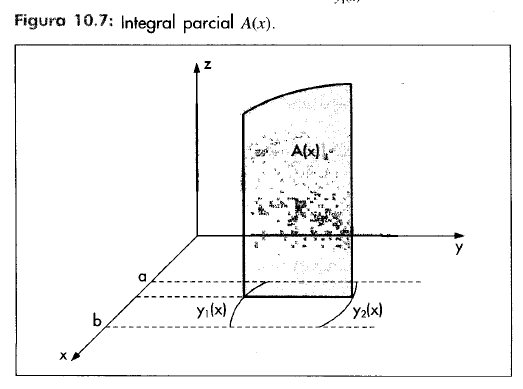
\includegraphics[height=7cm]{images/morettin_figura-10-7}
			\end{figure}

			No $2^{o}$ passo, o volume sob o gráfico e acima do domínio $D$, é dado por

			\medskip

			$V = \int \limits^{b}_{a} A(x)dx$ .

			\medskip

			Portanto, a integral dupla de $f(x, y)$ em $D$ é dada por

			\medskip

			$\iint_{D} f(x, y)dxdy = \int \limits^{b}_{a} \left[ \int \limits^{y_{2}(x)}_{y_{1}(x)} f(x, y)dy \right] dx$ .

			\bigskip

			\textbf{Exemplo}. Seja $f(x, y) = 1$ e $D$  a região dada pelas inequações $0 \leq x \leq 1$ e $x^{2} \leq y \leq x$. Calculemos o volume sólido sob o gráfico da função acima de $D$.

			A região $D$ é dada pela Figura 10.8.

			\begin{figure}[H]
				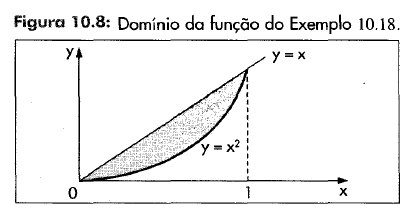
\includegraphics[height=5cm]{images/morettin_figura-10-8}
			\end{figure}

			Temos

			\medskip

			$A(x) = \int \limits^{x}_{x^{2}} 1dy = [y]^{x}_{x^{2}} = x - x^{2}$ ,

			$V = \int \limits^{1}_{0} (x - x^{2})dx = \left[ \cfrac{x^{2}}{2} - \cfrac{x^{3}}{3} \right]^{1}_{0} = \cfrac{1}{2} - \cfrac{1}{3} = \cfrac{1}{6}$ .

			\bigskip

			Uma terceira situação que ocorre no cálculo da integral dupla é aquela em que o domínio $D$ de $f(x, y)$ é dado por

			\medskip

			$c \leq y \leq d$

			\smallskip

			e

			\smallskip

			$x_{1}(y) \leq x \leq x_{2}(y)$

			\medskip

			Veja a Figura 10.9

			\begin{figure}[H]
				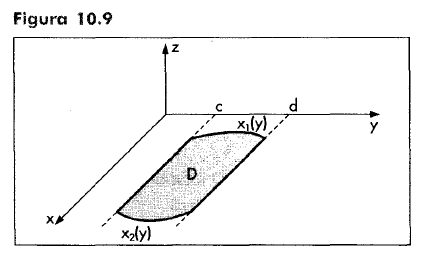
\includegraphics[height=5.5cm]{images/morettin_figura-10-9}
			\end{figure}

			O $1^{o}$ passo para calcular a integral dupla consiste em achar a área $B(y)$ de uma secção do gráfico da função perpendicular ao eixo $y$. Isto é

			\medskip

			$B(y) = \int \limits^{x_{2}(y)}_{x_{1}(y)} f(x, y)dx$ (Figura 10.10).

			\begin{figure}[H]
				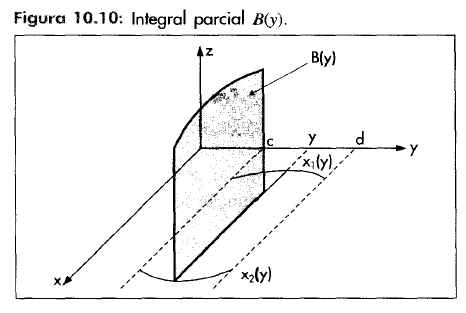
\includegraphics[height=7cm]{images/morettin_figura-10-10}
			\end{figure}

			O $2^{o}$ passo consiste em calcular o volume sob o gráfico de $f(x, y)$ e acima $D$, por meio da integral

			\medskip

			$V = \int \limits^{d}_{c} f(x, y)dy$ .

			\medskip

			Portanto, a integral dupla de $f(x, y)$ em $D$ é dada por

			\medskip

			$\iint_{D} f(x, y)dxdy = \int \limits^{d}_{c} \left[ \int \limits^{x_{2}(y)}_{x_{1}(y)} f(x, y)dx \right] dy$ .

			\bigskip

			\textbf{Exemplo}. Consideremos a função $f(x, y) = x + y$ e calculemos a integral dupla $\iint_{D} f(x, y)dxdy$, em que a região $D$ é dada por

			\medskip

			$1 \leq y \leq 2$

			\smallskip

			e

			\smallskip

			$y \leq x \leq 3y$ .

			\medskip

			Temos

			\medskip

			$B(y) = \int \limits^{3y}_{y} (x + y)dx = \left[ \cfrac{x^{2}}{2} + xy \right]^{3y}_{y} = \cfrac{9y^{2}}{2} + 3y^{2} - \cfrac{y^{2}}{2} - y^{2} = 6y^{2}$ ,

			$V = \int \limits^{2}_{1} 6y^{2}dy = [2y^{3}]^{2}-{1} = 2 \times (8) - 2 \times (1) = 14$ .

			\medskip

			Portanto, a integral dupla procurada vale 14.

			\bigskip

			\textbf{Observações}

			\begin{enumerate}[label=\alph*)]

				\item De modo geral, se o domínio $D$ não puder ser expresso de acordo com as situações descritas, então subdividimos o domínio em partes tais que cada uma se enquadre nos casos dados.

				\item Nos casos estudados, consideramos $f(x, y) \geq 0$; caso tenhamos $f(x, y) \leq 0$, então $-f(x, y) \geq 0$. Assim, a integral dupla da função será o oposto do volume do sólido compreendido entre $D$ e o gráfico da função.
				
			\end{enumerate}